% Compile like this, adjusting filenames as needed.
% Compile: perl compile-thesis-from-scratch.pl compile-opts.tex
% Compile: xelatex  -jobname thesis  compile-opts.tex

% Edit compile options here to support current active file compilation using Latex Workshop
% To use any of them, just uncomment it
% \newcommand*\optCommittee{}%   碩士論文合格證明書(中英)
% \newcommand*\optHyperlinks{}%  超連結，列印紙本紙不要用
% \newcommand*\optWatermark{}%   浮水印很難看，除了學校要求的時候以外不要用

\documentclass[BibLaTeXsortingNone]{PHlab-thesis}

\addbibresource{thesis.bib}

\newcommand*\DepartmentTW{資訊工程學系}
\newcommand*\DepartmentEN{Department of Computer Science and Information Engineering}

\newcommand*\fullModelName{nn\sout{M}Net} % Feel free to delete it after changing the title
\newcommand*\ThesisTitleTW{\fullModelName{}: 火星地形語意分割基準模型}
\newcommand*\ThesisTitleEN{\fullModelName{}: Baseline for Martian Terrain Semantic Segmentation}
% \newcommand*\ThesisNoteTW{初稿}% For real thesis omit, or use {初稿} etc.
% \newcommand*\ThesisNoteEN{draft}% For real thesis omit, or use {draft} etc.

\newcommand*\StudentTW{李明翰}
\newcommand*\StudentEN{Ming-Han Lee}

\newcommand*\AdvisorTW{陳奇業}
\newcommand*\AdvisorEN{Chi-Yeh Chen}

% 如果有共同指導老師可以用:
% \newcommand*\CoAdvisorATW{}
% \newcommand*\CoAdvisorAEN{}
% \newcommand*\CoAdvisorBTW{}
% \newcommand*\CoAdvisorBEN{}

\newcommand*\YearMonthEN{July, 2026}
\newcommand*\YearMonthTW{一一五年七月}

% Replace fancy with plain to get rid of fancyhdr because it's a little bit messy
% \pagestyle{fancy}% Use fancyhdr
\pagestyle{plain}

\hyphenation{Wiki-pedia} % For syllabification at the end of the line
% \setmathfont{TeX Gyre Termes Math} % A nice looking math font

\begin{document}

%   As much as possible, the abstract should be stand alone.
%   Many people will read only the abstract, not the main paper.
%   In fact after publication somtimes only the abstract is visable (on the University webpage for example?)
%
%   So it is worth the effort to write a good abstract.  中文的摘要也要寫的好!
%
%   In order to make the abstact be readable independent of the rest of the thesis.
%
%   1. In the abstact, citations should be kept to a minimum.
%   But sometimes it makes sense to cite one or two key papers in the abstract
%   In that case, write the authors names out, as in:
%
%      Sequence logos (Schneider \& Stephens, NAR, 1990)
%
%   Instead of using \cite{SS90}, which would produce a numerical cite like:
%
%      Sequence logos [4]   <--  [4] here is not useful when viewing only the abstract.
%
%
%   2. Abbreviations should be kept to a minimum, and if necessary defined in the abstract.
%
%   For example a student once used "CoOp-based prompt learning" in an abstract;
%   where "CoOp" stands for "Context Optimization".
%   "CoOp" was defined in the nomenclature section, so no problem with using it the main text.
%
%   But the abstract should be not rely on the nomenclature section, so in this case
%   it would be better to use "Context Optimization based prompt learning" in the abstract,
%   in other words avoid the abbreviation altogehter.
%
%   Sometimes it is okay to use abbreviations in the abstract, but define then when first used.
%   Exceptions would be nearly universally known abbreviations such as "DNA" for DeoxyriboNucleic Acid.
%   What is considered "Nearly universally known" may vary from person to person
%   － when in doubt assume some readers may not know.
%
%   Actually, in the example abstract below is not a good example in this sense.
%   It is from a research article in a specialized journal and contains several protein names:
%   MYC, CEBPB, and ZBTB33.
%   These are in some sense abbreviations, but usually treated just as names.
%   There is also another special abbreviation CpG.
%   Note that I at least try to give a hint about them;
%   for example "transcription factor MCY" and "CpG dimer".

\newcommand*\KeywordsEN{keyword1, keyword2, keyword3}
\newcommand*\AbstractEN{%
  Your abstract.}


\newcommand*\KeywordsTW{關鍵詞1、關鍵詞2、關鍵詞3}
\newcommand*\AbstractTW{%
  你的摘要。
}


\newcommand*\Acknowledgements{%
  你的致謝。
  \noindent
  \hspace*{\fill} \\

  \hfill \begin{tabular}{ll}
    李明翰    & 謹誌於          \\
    國立成功大學 & 資訊工程學系       \\
    中華民國   & \YearMonthTW\end{tabular}
}


% ---------------------------------------------------------------------------- %
%                                 Configuration                                %
% ---------------------------------------------------------------------------- %
%% Note the double {{ }}, this grouping contains the fontsize change to the scope of the macro.
%% These two macros set \baselineskip 2pt more than the fontsize, represented by #1
\newcommand*\SelectFontsizeMD[2]{{\fontsize{#1}{\numexpr #1 + 2}\selectfont\mdseries#2\par}}
\newcommand*\SelectFontsizeBF[2]{{\fontsize{#1}{\numexpr #1 + 2}\selectfont\bfseries#2\par}}

\newcommand*\SignatureRule[1][6]{\rule{#1cm}{0.3mm}}
\newcommand*\AddToContents[1]{\newpage\phantomsection\addcontentsline{toc}{chapter}{#1}}

\doublespace
\pagenumbering{gobble}% Turn off page numbering.
\renewcommand{\thefootnote}{\fnsymbol{footnote}}

\newgeometry{tmargin=2.3cm, bmargin=3cm, lmargin=2cm, rmargin=2cm}


% ---------------------------------------------------------------------------- %
%                                     Cover                                    %
% ---------------------------------------------------------------------------- %
\begin{center}
  \vspace{2cm}
  \SelectFontsizeBF{24}{%
    \UniversityTW\DepartmentTW\\
    \Degree 論文}

  \vfill
  \SelectFontsizeBF{24}{\ThesisTitleTW}
  \ifdefined\ThesisNoteTW
    \SelectFontsizeMD{22}{\textit{\ThesisNoteTW}}
  \fi

  \vspace{5mm}
  \SelectFontsizeBF{22}{\ThesisTitleEN}
  \ifdefined\ThesisNoteEN
    \SelectFontsizeMD{20}{\textit{\ThesisNoteEN}}
  \fi

  \vfill
  \begin{minipage}{\linewidth}
    \centering
    \SelectFontsizeMD{20}{%
      \begin{tabular}{ r r @{\hspace{2em}} l l }
        研究生：  & \StudentTW    & Student:    & \StudentEN    \\
        指導老師： & \AdvisorTW    & Advisor:    & \AdvisorEN    \\
        \ifdefined\CoAdvisorATW
        共同指導： & \CoAdvisorATW & Co-Advisor: & \CoAdvisorAEN \\
        \fi
        \ifdefined\CoAdvisorBTW
              & \CoAdvisorBTW & Co-Advisor: & \CoAdvisorBEN \\
        \fi
      \end{tabular}}
  \end{minipage}

  \vfill
  \SelectFontsizeMD{18}{%
    \DepartmentEN,\\
    National Cheng Kung University,\\
    Tainan, Taiwan, R.O.C.\\
    Thesis for \ifdef\PhD{Doctor of Philosophy}{Master of Science} Degree\\
    \YearMonthEN}

  \vfill
  \SelectFontsizeMD{20}{中華民國\YearMonthTW}
\end{center}

\restoregeometry


% ---------------------------------------------------------------------------- %
%                                  Certificate                                 %
% ---------------------------------------------------------------------------- %
\ifdefined\optCommittee
  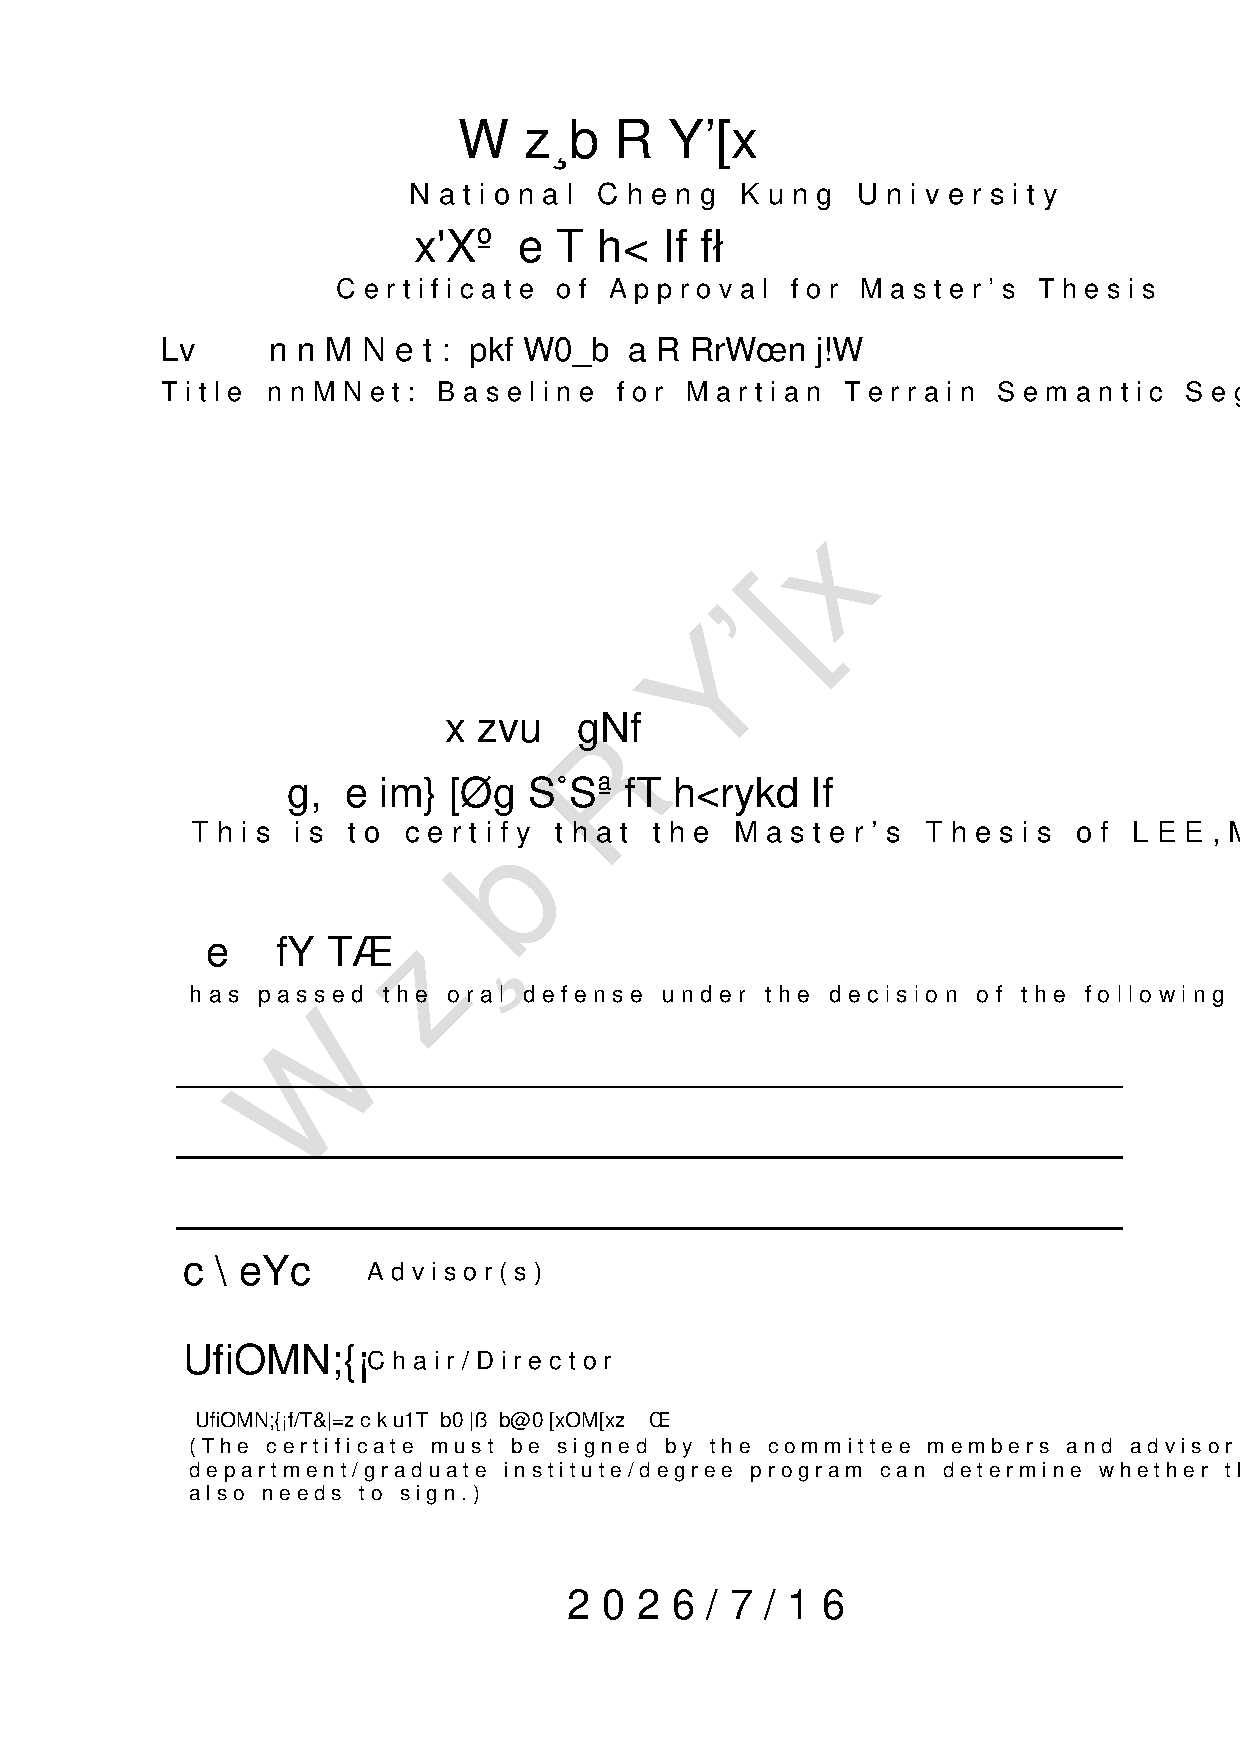
\includepdf[pages={1}]{certificate.pdf}
\fi


% ---------------------------------------------------------------------------- %
%                              Abstract (Chinese)                              %
% ---------------------------------------------------------------------------- %
\AddToContents{中文摘要}
\setcounter{page}{1}
\pagenumbering{roman}

\begin{center}
  \SelectFontsizeBF{24}{\ThesisTitleTW}

  \vspace{4mm}
  \SelectFontsizeMD{18}{\StudentTW\footnote[1]{學生} ~ \AdvisorTW\footnote[2]{指導教授}}

  \vspace{5mm}
  \SelectFontsizeMD{20}{國立成功大學\DepartmentTW}

  \vspace{12mm}
  \makebox[2.7cm][c]{\SelectFontsizeBF{22}{摘要}}
\end{center}

\vspace{4mm}
\SelectFontsizeMD{12}{\AbstractTW}

\vspace{4mm}
\begin{flushleft}
  \SelectFontsizeMD{12}{關鍵詞: \KeywordsTW}
\end{flushleft}

% ---------------------------------------------------------------------------- %
%                              Abstract (English)                              %
% ---------------------------------------------------------------------------- %
\AddToContents{Abstract}
\begin{center}
  \SelectFontsizeBF{22}{\ThesisTitleEN}

  \vspace{4mm}
  \SelectFontsizeMD{18}{\StudentEN\footnote[1]{Student} ~ \AdvisorEN\footnote[2]{Advisor}}

  \vspace{4mm}
  \SelectFontsizeMD{16}{\DepartmentEN, National Cheng Kung University}

  \vspace{12mm}
  \SelectFontsizeBF{20}{Abstract}
\end{center}

\vspace{4mm}
\SelectFontsizeMD{12}{\AbstractEN}

\vspace{4mm}
\begin{flushleft}
  \SelectFontsizeMD{12}{Keywords: \KeywordsEN}
\end{flushleft}


% ---------------------------------------------------------------------------- %
%                               Acknowledgements                               %
% ---------------------------------------------------------------------------- %
\ifdefined\Acknowledgements
  \AddToContents{誌謝}
  \begin{center}\SelectFontsizeBF{24}{誌謝}\end{center}

  \vspace{4mm}
  \Acknowledgements
\fi


% ---------------------------------------------------------------------------- %
%                                   Contents                                   %
% ---------------------------------------------------------------------------- %
\renewcommand{\contentsname}{Contents}
\AddToContents{Contents}
\tableofcontents

\AddToContents{List of Tables}
\listoftables

\AddToContents{List of Figures}
\listoffigures
% 封面頁, 口委中英文簽名單, 誌謝, 中英文摘要, 論文目錄, 圖表目錄


% Nomenclature, FYR
% \renewcommand\nomgroup[1]{%
%   \item[\bfseries
%   \ifstrequal{#1}{A}{General}{%
%   \ifstrequal{#1}{Z}{Gene/Protein Names}%
%   }]}

% \nomenclature[A]{$\lg$}{Logarithm base 2}
% \nomenclature[A]{KL Divergence}{Kullback-Liebler Divergence}
% \nomenclature[A]{ChIP}{Chromatin ImmunoPrecipitation}
% \nomenclature[Z]{CEBPB}{CCAAT/Enhancer-Binding Protein Beta}
% \nomenclature[Z]{Myc}{MYC proto-oncogene}
% \nomenclature[Z]{USF-1}{Upstream stimulatory factor 1}

% \printnomenclature[5cm]% Width of first field in Nomenclature; adjust as necessary.

\newpage
\setcounter{page}{1}
\pagenumbering{arabic}


\chapter{Introduction}
Your introduction.
% You can use \textcite or ~\cite to cite references.
% The ~ here is a special kind of space which ensure no line break between "depth" and the citation number.
\textcite{SS90} introduced sequence logos many years ago.
The seminal results of Erwin Schrödinger~\cite{Sch26} are not directly relevant.


\chapter{Related Work}
Your related work.


\chapter{Method}
Your method.


\section{Mathematical Model}
\subsection{Notation}
The notation used in this thesis is summarized in table~\ref{tab:notation}.

\subsection{Likelihood Calculation}
Our model assumes the data follows a standard normal distribution $𝒩(μ,σ²)$, so the likelihood function is:

\begin{align*}
  ℒ  \;= & \;\;  \frac{1}{σ\sqrt{2π}}\, \exp\Big( \frac{-(x-μ)²}{2σ²}\Big)              \\[.5ex]% .5ex adds extra vertical height
  ∝      & \;\;  σ⁻¹\, \exp\big( -½\,z²)  \hspace{1cm} \text{where~~} z ≝ \frac{x-μ}{σ}
\end{align*}


\begin{table}
  \begin{tabularx}{0.9\linewidth}{lX}
    Notation                                            & Description                                                                                                                        \\
    \toprule
    $P_{\text{meth}\,|\,\textsf{context,BG}}$           & The background probability of methylation by context.                                                                              \\[.3ex]
    $n_{\textsf{context},\,i}$                          & The number of cytosines (with sufficient read coverage)\newline of the given context occurring at position $i$ in the set of TFBS. \\[.3ex]
    $\overline{v}\,|\,\scriptstyle{\textsf{context},i}$ & The average methylation values of those cytosines.                                                                                 \\
    \bottomrule
  \end{tabularx}
  \caption{Summary of notation used in this thesis.}
  \label{tab:notation}
\end{table}


% For long section names use: \section[short]{longer...} to make header look better.
% When given, the optional [short] argument is used for headers.
\section[Shorter Section Name]{Section name which is too long to fit in the header}


\section{Proposed Scheme}
Write a bunch of stuff here.

We propose the following items:
%
\begin{itemize}
  \item This is the first item we propose.
  \item And this is the second.
  \item But don't for get the third one!
\end{itemize}


\chapter{Experiments}
Your experiments and their results.


% Your discussion and future work, could be merged with the conclusion chapter.
% \chapter{Discussion}
% \chapter{Future Work}


\chapter{Conclusion}
Your conclusion.


\newpage
\AddToContents{References}
\printbibliography[title={References}]
\end{document}
